\documentclass[12pt]{article}   % you have 10pt, 11pt, or 12pt options

\setlength{\textwidth}{17.2cm}     % if you change this, consider changing
\setlength{\evensidemargin}{-.3cm} % side margins to retain centering
\setlength{\oddsidemargin}{-.3cm}

\setlength{\textheight}{23cm}   % if you change this, consider changing
\setlength{\topmargin}{-2cm}  % top margin to retain centering
\setlength{\headsep}{1.6cm}

%---------------------- These packages below add functionality to your version of LaTeX --------------
%---------------------- You might not use all of them --------------------------------------
\usepackage{amssymb}
\usepackage{latexsym}
\usepackage{amsthm}
\usepackage{enumerate}
\usepackage{epsfig}
\usepackage{graphicx}
\usepackage{color}
\usepackage{float}
\usepackage{subfig}
\usepackage{amsmath}
\usepackage{makeidx}
\usepackage{fancyhdr}
\pagestyle{fancy}
\usepackage{lastpage}
\usepackage{url}
\usepackage{algorithm}
\usepackage{algorithmic}
\usepackage[algo2e]{algorithm2e}
\usepackage{appendix}
\usepackage{bm}
\usepackage[utf8]{inputenc}
\usepackage[T1]{fontenc}
\usepackage{lmodern} % load a font with all the characters
%------------------------- Customized Header --------------------------------------------------------
\fancyhead{}
\fancyfoot{}			
\lhead{IMU + Camera}
\rhead{Page \thepage\ of \pageref{LastPage}}

%---------- the symbols below will give you the blackboard bold of R, T, etc. ----------
\DeclareSymbolFont{AMSb}{U}{msb}{m}{n}  
\DeclareMathSymbol{\Sph}{\mathbin}{AMSb}{"53} \DeclareMathSymbol{\R}{\mathbin}{AMSb}{"52}
\DeclareMathSymbol{\T}{\mathbin}{AMSb}{"54} \DeclareMathSymbol{\Z}{\mathbin}{AMSb}{"5A}
\DeclareMathSymbol{\K}{\mathbin}{AMSb}{"4B}

%------------------------- Theorem and Proof Environments -------------------------------------------------

% This section defines all the environments you might use.  Just type
% \begin{theorem, or corollary, or whatever}, then the optional name of the
% theorem inside {} (or empty {} if no name), then body of the theorem,
% corollary, whatever, also inside {} then \end{theorem, corollary, whatever}
%
% Notice when I use them in the paper, I put an optional "argument" to the function
% and this gives a name to the theorem

\newenvironment{theorem}[1]{\vspace{.9cm}\noindent    {\bf Theorem {#1}}}{\vspace{.1cm}}
\newenvironment{lemma}[1]{\vspace{.9cm}\noindent    {\bf Lemma {#1}}}{\vspace{.1cm}}
\newenvironment{corollary}[1]{\vspace{.9cm}\noindent    {\bf Corollary {#1}}}{\vspace{.1cm}}
\newenvironment{definition}{\vspace{.9cm}\noindent {\bf Definition}}{\vspace{.1cm}}
\def\qed{\hfill $\Box$}
\renewenvironment{proof}{\vspace{.5cm}   \noindent{\bf Proof: }}{\qed \vspace{1cm}}
 
%\theoremstyle{definition}
%\newtheorem{notation}[theorem]{Notation}
%\newtheorem{properties}[theorem]{Properties}
%\newtheorem{remark}[theorem]{Remark}
%\newtheorem{example}[theorem]{Example}
%\newtheorem{claim}[theorem]{Claim}
%\newtheorem{observation}[theorem]{Observation}
%\newtheorem{definition}[theorem]{Definition}


% ---------------------- Define case environment ------------------------------

\newcounter{case}

\newenvironment{case}[1]{\stepcounter{case} \addvspace{.5\baselineskip} \noindent\textbf{Case \thecase}. \textit{#1}}{\hfill\fbox{Case \thecase}}

%\newtheorem{case}{Case}
\newtheorem{subcase}{Case}[case]
\newtheorem{sub2case}{Case}[subcase]
%\newtheorem{sub3case}{Case}[sub2case]
%\newtheorem{sub4case}{Case}[sub3case]


%Picture inclusion

\newcommand\pic[3]{
\begin{figure}[H] \begin{center} 
\epsfig{file=#1, height=#2pt} 
\end{center} 
\caption{#3} 
\end{figure}
}

\def\inj{\text{inj}}
\def\diam{\text{diam}}
\def\area{\text{area}}
\def\length{\text{length}}


\begin{document}  % necessary part of document


\title{Visual Inertial SLAM using Inertial Preintegration}
\author{Liyang Liu}
\date{\today}

\maketitle

\begin{abstract}
This document is a report on Visual Inertial SLAM using an efficient method of IMU pre-integration. The pre-integration method combines many IMU data as a single observation before fusion with camera images, resulting in a much reduced state and observation graph structure. An accurate map and robot path is hence obtainable in real-time. We present the pre-integration theory, including formulation of motion state, observation, uncertainty, observation model and the Jacobians. We provide an implementation, compare the performance difference for VIN systems with and without pre-integration. We also include a discussion of various initialization setups along with their impact on linearization of the original problem. Based on our experimental results, we propose future research plans.
\end{abstract}

\newpage

\tableofcontents

\newpage

\section{Introduction}

\vspace{1cm}
In this work, we firstly simulate a navigation system equipped with an IMU and an RGB camera. 
\begin{figure}[ht]
	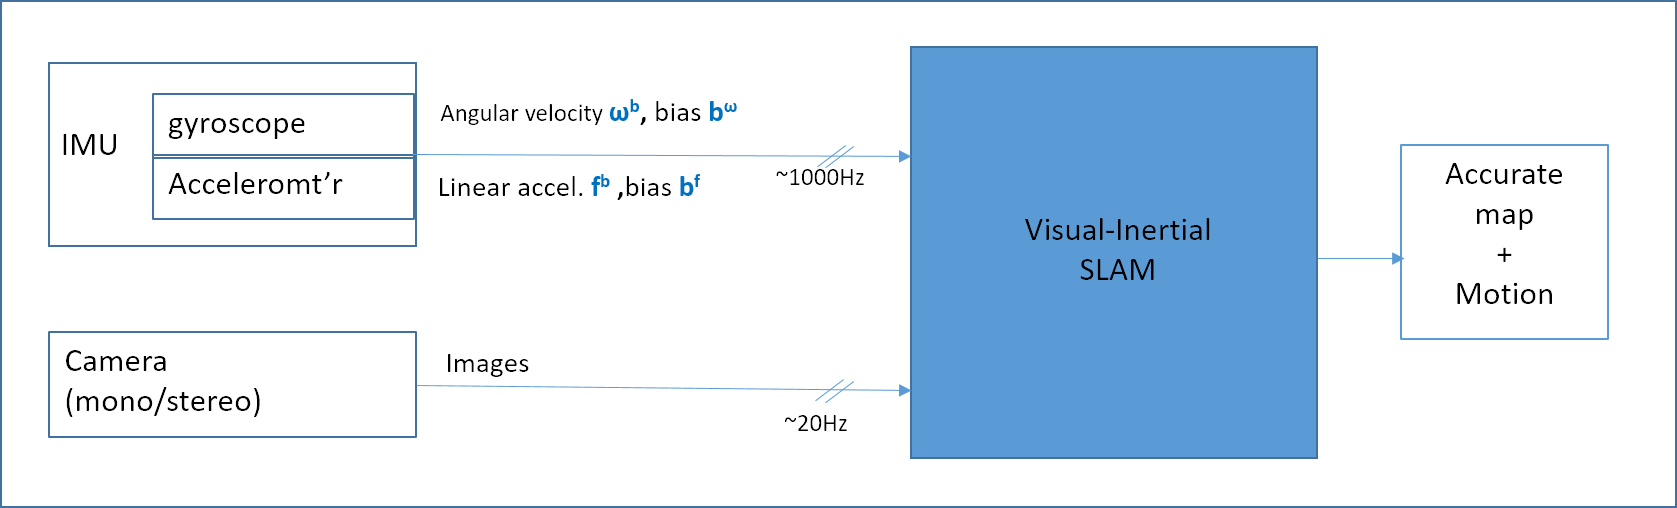
\includegraphics[height=5cm]{figures/VIN_block-diagram.png}
	\caption{VIN SLAM}
	\label{fig:vin}
\end{figure}

\paragraph{States}
The estimated state vector contains the 3-D vehicle position $\bm{p}^{\mathrm{n}}$, velocity $\bm{v}^{\mathrm{n}}$ and Euler angles $\bm{A}^{\mathrm{n}}=[\alpha,\beta,\gamma]$; as well as the M feature locations ($\bm{f}_i^{\mathrm{n}}$) in the environment where i = 1,...N. 
\paragraph{Sensor data}
The IMU readings include 3-D linear acceleration $\bm{f}^{\mathrm{b}}$ and angular rate $\bm{\omega}^{\mathrm{b}}$, both given in body frame and come with non-zero bias : $\bm{b}_f$ and $\bm{b}_\omega$. \newline
Further, due to its design principal, the IMU can only measure acceleration with the gravity taken out, therefore the true vehicle's acceleration in the world frame should be \\
$\bm{f}^{\mathrm{n}} = R_b^{\mathrm{n}}( \bm{f}^{\mathrm{b}}-\bm{b}_f ) + \bm{g}^{\mathrm{n}}$ \\
$R_b^{\mathrm{n}}$ and $E_b^{\mathrm{n}}$ are the rotation and rotation rate matrices.
Superscript refers to the reference frame, ${}^{\mathrm{n}}$ is the navigation frame.

\paragraph{The Original VIN model}
The motion model based on IMU reading can be stated as
\begin{align*}
	\triangle t & =  t_{t+1} - t_t \\
	\bm{f}_t^{\mathrm{n}} & = R_{bt}^{\mathrm{n}}  (\bm{f}_t^{\mathrm{b}} - \bm{b}_f) \\
	\bm{v}_{t+1} & = \bm{v}_{t} + \bm{f}_t^{\mathrm{n}} \triangle t + \bm{g}^{\mathrm{n}} \triangle t \\
	\bm{p}_{t+1} & = \bm{p}_{t} + \bm{v}_t \triangle t \\
	\bm{A}_{t+1} & = \bm{A}_t + E_{bt}^{\mathrm{n}}  (\bm{\omega}_t^{\mathrm{b}} - \bm{b}_\omega) \triangle t
\end{align*}

\section{The original VIN problem}
For a system composed of an IMU and a RGB camera navigating with $N$ camera poses, $K$ IMU samples per image and $M$ features. The naive VIN problem includes robot poses at all IMU sample times.

\paragraph{State Vector}
the state vector $\textbf{X}$ is defined as:
\begin{align*}
\textbf{x} = &(\overbrace{\textbf{A}_{10}, \textbf{p}_{10}, \textbf{A}_{20}, \textbf{p}_{20},... ,\textbf{p}_{K-1,0}, \textbf{p}_{K-1,0},\textbf{A}_{0,1}, \textbf{p}_{0,1},...,\textbf{A}_{K-1,1}, \textbf{p}_{K-1,1},... \textbf{A}_{K-1,N-1}, \textbf{p}_{K-1,N-1},\textbf{A}_{0N}, \textbf{p}_{0N}}^{K \times (N - 1) \ {\mathrm{ poses}}},\\
	 &\overbrace{\textbf{F}_{1},\textbf{F}_{2}, ..., \textbf{F}_{M}}^{M \ {\mathrm{ features}}},\\
	 &\overbrace{\textbf{v}_{00},\textbf{v}_{10} ...,\textbf{v}_{K-1,0}, ...,\textbf{v}_{0,N-1},...,\textbf{v}_{K-1,N-1}, \textbf{v}_{0N}}^{(K \times (N-1)+1)  \ {\mathrm{ velocities}}},\\
	 &\textbf{g}^{\mathrm{n}}, \textbf{A}_{u2c}, \textbf{T}_{u2c}, \textbf{b}_f, \textbf{b}_w )' 
\end{align*}

\paragraph{Observation Vector}
The Observation vector $\textbf{Z}$ is defined as:

\begin{align}
\textbf{z}_{raw} &= (\textbf{z}_{camera}, \textbf{z}_{IMUraw}, \textbf{z}_{Tv})' \nonumber \\
=& (\overbrace{\textbf{uv}_{11}, \textbf{uv}_{21}, ... , \textbf{uv}_{M1}, ..., \textbf{uv}_{1N}, \textbf{uv}_{2N}, ... , \textbf{uv}_{MN}}^{M \times N \ {\mathrm{pixels}}}, \nonumber \\ 
& \overbrace{\omega\textbf{f}_{01}, \omega\textbf{f}_{11}, ... , \omega\textbf{f}_{(K-1)1}, ..., \omega\textbf{f}_{0(N-1)}, \omega\textbf{f}_{1(N-1)}, ... , \omega\textbf{f}_{(K-1)(N-1)}}^{K \times (N-1) \ {\mathrm{IMU \ readings}}}, \\
& \overbrace{\textbf{0}, \textbf{0}, ... , \textbf{0}}^{K \times (N-1)  \ {\mathrm{ zero \ contraints}}})' 
\end{align}

See Appendix \ref{apn:naiveVin} for details on Naive VIN motion model and optimization details.
Clearly, such a large state space quickly becomes difficult to manage in practice. Further, each step of re-linearization, the integration from acceleration to velocity then to position has to be recomputed.

\section{The Preintegration algorithm}

\begin{figure}[!h]
	\begin{center}\begin{tabular}{cc}
			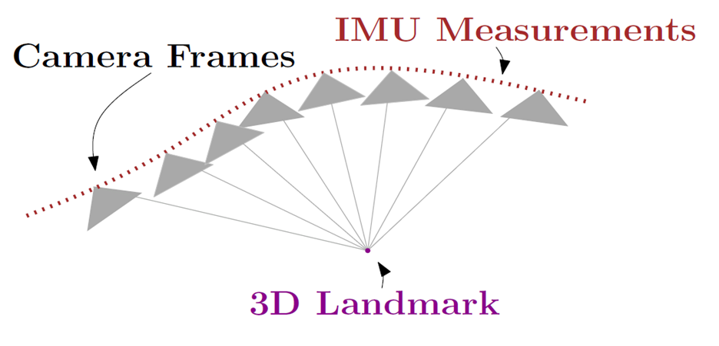
\includegraphics[height=3.3cm]{figures/IMU-sample_Image-frames_3D_illustration.png}&
			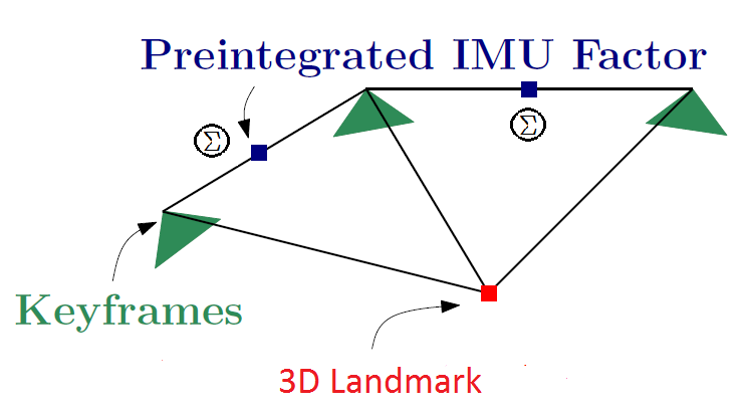
\includegraphics[height=3.3cm]{Figures/Preintegrated-IMU_image_3D_illustration.png}\\
			(a) & (b) \\
		\end{tabular}\end{center}
		\caption{\emph{a}) Samples: Camera+IMU \emph{b}) Inertial-delta: preintegrated information \cite{Manifold2015}} 
		\label{fig:VIN sensor information}
	\end{figure} 
Todd Lupton proposed the Preintegration method in 2012 \cite{Lupton2012}: integrate a large number of high rate IMU observations into a single observation, making it faster and easier to deal with in a SLAM or navigation filter. IMU data are integrated in a body fixed frame that moves with the vehicle, transformation to navigation frame only happens at end of integration, hence the algorithm is referred to as Pre-Integration.

The navigation frame in Preintegration VIN is defined as the body frame at initial robot pose, instead of the traditional globally referenced frame.

With a stereocamera, Todd Lupton also provided a way to recover the absolute global frame after 3 images of observation. However this is not possible with monocular camera setup.

\paragraph{Inertial Delta observation} The integrated term, including position, velocity and attitude is referred to as inertial delta observation $\triangle \bm{I}$.

\paragraph{Motion from Inertial Delta}
Relationship between robot motion state to inertial delta is shown in Equations (\ref{eq:Idt2X_orig_1} - \ref{eq:Idt2X_orig_3})
\begin{align}
\bm{p}^{\mathrm{n}}_{t2} = & \bm{p}^{\mathrm{n}}_{t1} + (t2 - t1) \bm{v}^{\mathrm{n}}_{t1} + 
\frac{1}{2} (t2 - t1 )^2 \bm{g}^{\mathrm{n}} + R^{\mathrm{n}}_{bt1} \triangle {\bm{p}^{t1}_{t2}}^+ 
\label{eq:Idt2X_orig_1}\\
\bm{v}^{\mathrm{n}}_{t2} = & \bm{v}^{\mathrm{n}}_{t1} + (t2 - t1 ) \bm{g}^{\mathrm{n}} + R^{\mathrm{n}}_{bt1} \triangle \bm{v}^{t1}_{t2} 
\label{eq:Idt2X_orig_2}\\
\bm{A}^{\mathrm{n}}_{t2} = & EulerFromDCM( R^{\mathrm{n}}_{bt1} \triangle R^{\mathrm{bt1}}_{bt2} )
\label{eq:Idt2X_orig_3}
\end{align}

\begin{algorithm}
	\caption{The Pre-integration Method Based on Inertial Raw Data}
	\label{algm:preint}		
	\begin{algorithmic}
	\STATE Inertial-delta observation $ \triangle \bm{\mathrm{I}} = \begin{bmatrix} \triangle \textbf{p}_{t}^+ \\ \triangle \textbf{v}_{t} \\ \triangle \textbf{A} _{t} \end{bmatrix}$, initially set to $\begin{bmatrix} 0 \\ 0 \\ 0 \end{bmatrix}$
		\FOR{$t_1 < t < t_2$}
		\STATE $\triangle t =  t_{t+1} - t_t$ 
		\STATE $\textbf{f}_t^{\mathrm{bt1}} = R_{\mathrm{bt}}^{\mathrm{bt1}} (\textbf{f}_t^{\mathrm{b}} - \textbf{b}_f)$ 
		\STATE $\triangle \textbf{v}_{t+1} = \triangle \textbf{v}_{t} + \textbf{f}_t^{\mathrm{bt1}} \triangle t$ 
		\STATE $\triangle \textbf{p}_{t+1}^+ = \triangle \textbf{p}_{t}^+ + \triangle \textbf{v}_t \triangle t$ 
		\STATE $\triangle \textbf{A} _{t+1} = \triangle \textbf{A} _{t} + E_{\mathrm{bt}}^{\mathrm{bt1}} (\omega _t^{\mathrm{b}} - \textbf{b}_\omega) \triangle t$ 
		\ENDFOR
	\end{algorithmic}
\end{algorithm}

\subsection{Formulation of Preintegration}
\paragraph{State Vector} $\textbf{X}_{prn}$ is defined as:
$$\textbf{X}_{prn} = (\overbrace{\textbf{A}^u_2, \textbf{p}^u_{2}, ... , \textbf{A}^u_{N}, \textbf{p}^u_{N}}^{N - 1 \ {\mathrm{ poses}}}, \overbrace{\textbf{F}_{1}, ..., \textbf{F}_{M}}^{M  \ {\mathrm{features}}}, \overbrace{\textbf{v}_1, ..., \textbf{v}_{N}}^{N \ {\mathrm{velocities}}},  \textbf{g}^{\mathrm{n}}, \textbf{A}_{u2c}, \textbf{T}_{u2c}, \textbf{b}_f, \textbf{b}_w)' $$
where
$\textbf{A}^u_i = (\alpha^u_i, \beta^u_i, \gamma^u_i)$,
$\textbf{p}^u_i = (x^u_i, y^u_i, z^u_i) $,
$\textbf{F}_{i} = (x_{i}, y_{i}, z_{i}) $.
\paragraph{Observation vector} becomes:

$$\textbf{Z}_{prn} = (\overbrace{\textbf{uv}_{1}, ... , \textbf{uv}_{N}, ..., \textbf{uv}_{1N}, ... , \textbf{uv}_{MN}}^{M \times N  \ {\mathrm{pixels}}}, \overbrace{\triangle \textbf{p}^+_2, \triangle  \textbf{v}_2, \triangle \textbf{A}_2, ..., \triangle  \textbf{p}^+_N, \triangle \textbf{v}_N, \triangle  \textbf{A}_N}^{N - 1 \ {\mathrm{inertialDeltas}}})' $$
where $\textbf{uv}_{ij} = (u_{ij}, v_{ij})$ represents the image of the $i$th feature point  at the $j$th camera pose.


\subsection{IMU bias}
Algorithm \ref{algm:preint} gives the pre-integration process model, it is therefore possible to compute is uncertainty from that of IMU measurements. Also, the IMU readings contain non-zero biase terms, so do not reflect the true motion's angular rate and acceleration. We tackle this problem in two steps, we assume $\bm{b}$ is known in computing inertial delta $\triangle \bm{I}$; then correct for the error in the optimization stage.

\subsubsection{Modified process model for Inertial-delta + Bias}
To analyze the effect of the unknown bias term on Inertial Delta observation, we modified the process model in Algorithm \ref{algm:preint} to include evolution of Inertial Delta plus bias. The expanded Inertial delta observation is denoted $\triangle I^+$, the new model is illustrated in algorithm \ref{algm:preintBias}
\begin{algorithm}
	\caption{The Pre-integration Method Based on Inertial Raw Data}
	\label{algm:preintBias}		
	\begin{algorithmic}
		\STATE Extended Inertial-delta observation $ \triangle \bm{\mathrm{I}}^+ = \begin{bmatrix} 
		\triangle \textbf{p}_{t}^+ \\
		\triangle \textbf{v}_{t} \\
		\triangle \textbf{A} _{t} \\
		\textbf{b}_f \\
		\textbf{b}_{\omega}
		\end{bmatrix}$, initially set to $\begin{bmatrix} 
		0 \\ 
		0 \\ 
		0 \\
		0 \\
		0
		\end{bmatrix}$
		%\begin{flalign*}
		%\STATE $\triangle \textbf{p}^+_t = 0$, $\triangle \textbf{v}_t = 0$, $\triangle \textbf{A}_t = 0$ 
		%\end{flalign*}
		\FOR{ $t_1 < t < t_2$ }
			\STATE $\triangle t =  t_{t+1} - t_t$ 
			\STATE $\textbf{f}_t^{\mathrm{bt1}} = R_{\mathrm{bt}}^{\mathrm{bt1}} (\textbf{f}_t^{\mathrm{b}} - \textbf{b}_f)$ 
			\STATE $\triangle \textbf{v}_{t+1} = \triangle \textbf{v}_{t} + \textbf{f}_t^{\mathrm{bt1}} \triangle t$ 
			\STATE $\triangle \textbf{p}_{t+1}^+ = \triangle \textbf{p}_{t}^+ + \triangle \textbf{v}_t \triangle t$ 
			\STATE $\triangle \textbf{A} _{t+1} = \triangle \textbf{A} _{t} + E_{\mathrm{bt}}^{\mathrm{bt1}} (\omega _t^{\mathrm{b}} - \textbf{b}_\omega ) \triangle t$ 
			\STATE $\textbf{b}_f = \textbf{b}_f$
			\STATE $\textbf{b}_{\omega} = \textbf{b}_{\omega}$
		\ENDFOR
	\end{algorithmic}
\end{algorithm}

\subsection{Inertial delta $\Sigma$ and Bias Jacobian}
In order to apply the SLAM optimization framework, we need to provide the inertial delta's uncertainty and variability due to bias (i.e. Jacobian due to biase). To achieve this, we interpret Algorithm \ref{algm:preintBias} as an EKF in its own. This EKF has a state vector defined as $\triangle \bm{I}^+_t$, it is recursively computed as a function of previous state vector $\triangle \bm{I}^+_{t-1}$ and IMU readings, summarized in equation below:
\begin{equation}
\triangle {\bm{I}}^+_t = \bm{f}( \bm{\triangle I^+_{t-1}}, \bm{f}^{\mathrm{b}}_{t}, \bm{\omega}^{\mathrm{b}}_{t})
\end{equation}


The integration process is recursive, therefore the inertial delta's uncertainty $\Sigma$ and Jacobian $J$ (now against both inertial delta and bias terms ) are computed recursively, starting with a zero uncertainty and an identity matrix in the beginning, as illustrated in Figure \ref{fig:preintBlock}

\begin{figure}[h!]
	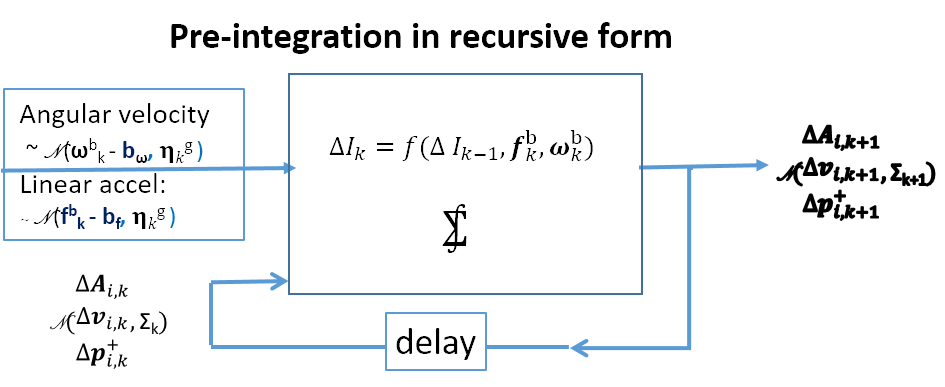
\includegraphics[height=6cm]{figures/Pre-integration_block-flow.png}
	\caption{Pre-Integration}
	\label{fig:preintBlock}
\end{figure}

In each discrete summation step, state covariance $\Sigma_t$ is related to the uncertainty $\Sigma_t$ at time $t-1$ (Fig \ref{fig:preintUncertainty}) and current measurement noise by $F_t$ and $G_t$, where $F_t$ and $G_t$ are the Jacobians of the state transition function $\bm{f}()$ w.r.t the state vector $\triangle I^+$ and the noise input $\mathrm{\bm{\eta}_t}$ respectively.
\begin{figure}[h!]
	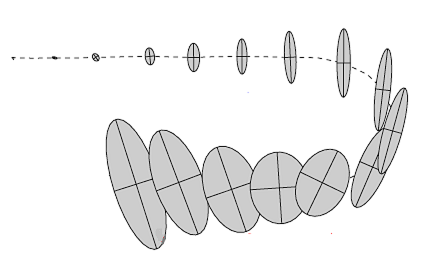
\includegraphics[height=7cm]{figures/Inertial-delta_covariance_evolution.png}
	\caption{Evolution of uncertainty during Pre-Integration}
	\label{fig:preintUncertainty}
\end{figure}

The modified process's Jacobian $J_{t}$ is a chain product of previous process's Jacobian $J_{t-1}$ and state transition Jacobian $F_{t-1}$. 
\begin{equation}
	\begin{split}
J^{t2}_{t1} =&\frac {\partial \triangle I^+_{t2}}{\partial \triangle I^+_{t1}}\\
= & \frac {\partial \triangle I^+_{t1+1}}{\partial \triangle I^+_{t1}} ... \frac {\partial \triangle I^+_{t2-1}}{\partial \triangle I^+_{t2-2}} . \frac {\partial \triangle I^+_{t2}}{\partial \triangle I^+_{t2-1}} \\
\end{split}
\end{equation}
The final structure of Jacobian $J^{t2}_{t1}$ is shown in Equation \ref{eq:IJB}. As the initial vehicle states are set to zero at the beginning of each delta, only the last two columns of this matrix, relating to the bias terms, are important for the result but the whole matrix is required for the internal calculations. The last 2 columns of the matrix is the Jacobian's bias component, it reflects how the inertial delta $\triangle \bm{I}$ changes versus the biasing terms. This will be useful in the subsequent VIN optimization process. The complete covariance and Jacobian calculation algorithm are listed in algorithm \ref{algm:preint_cov}. \\


\begin{algorithm}[h!]
	\caption{The Covariance Matrix for the Pre-integration Method}
	\label{algm:preint_cov}
	\begin{algorithmic}%[8]
		%\begin{flalign*}
		\STATE $J_t = \textbf{I}_{15}$ 
		\STATE ${\Sigma}_t = \textbf{I}_{15}$ 
		\FOR{$t_1 < t < t_2$}
		\STATE $\triangle t =  t_{t+1} - t_t$ 
		\STATE $\alpha = \frac{d R^{\mathrm{bt1}}_{\mathrm{bt}} (\textbf{f}_t - \textbf{b}_f)}{d \textbf{A}_t}$
		\STATE $\beta = \frac{d E^{\mathrm{bt1}}_{\mathrm{bt}} (\omega_t - \textbf{b}_\omega)}{d \textbf{A}_t}$
		\STATE $F_t = \begin{bmatrix} \textbf{I}_3 & \textbf{I}_3 \triangle t & \textbf{0}_3 & \textbf{0}_3 & \textbf{0}_3 \\ 
		\textbf{0}_3 & \textbf{I}_3  & \alpha \triangle t & -R^{\mathrm{bt1}}_{\mathrm{bt}} \triangle t & \textbf{0}_3 \\ 
		\textbf{0}_3 & \textbf{0}_3 & \textbf{I}_3 + \beta \triangle t & \textbf{0}_3 & -E^{\mathrm{bt1}}_{\mathrm{bt}} \triangle t \\
		\textbf{0}_3 & \textbf{0}_3 & \textbf{0}_3 & \textbf{I}_3 & \textbf{0}_3 \\
		\textbf{0}_3 & \textbf{0}_3 & \textbf{0}_3 & \textbf{0}_3 & \textbf{I}_3
		\end{bmatrix}$
		\STATE $G_t = \begin{bmatrix} \textbf{0}_3 & \textbf{0}_3 \\ R^{\mathrm{bt1}}_{\mathrm{bt}} \triangle t & \textbf{0}_3 \\ \textbf{0}_3 & E^{\mathrm{bt1}}_{\mathrm{bt}} \triangle t \\ \textbf{0}_3 & \textbf{0}_3 \\ \textbf{0}_3 & \textbf{0}_3 \end{bmatrix}$
		\STATE $J_{t+1} = F_{t} J_t$ 
		\STATE ${\Sigma}_{t+1} = F_{t} {\Sigma}_t F'_{t} + G_t Q_t G'_t$ 
		\ENDFOR
		\STATE $J^{t2}_{t1} = J_{t}$
		\STATE ${\Sigma}^{t2}_{t1} = {\Sigma}_{t}$
	\end{algorithmic}
\end{algorithm}

\begin{equation}
J=\begin{bmatrix}
\frac{\partial { \triangle \bm{p}^+_{t2}}}{\partial \bm{p}^{t1}_{t1}}		&	
\frac{\partial { \triangle \bm{p}^+_{t2}}}{\partial \bm{v}^{t1}_{t1}}		& 
\frac{\partial { \triangle \bm{p}^+_{t2}}}{\partial \bm{A}^{t1}_{t1}}		&
\frac{\partial { \triangle \bm{p}^+_{t2}}}{\partial \bm{b}_{f}}		&
\frac{\partial { \triangle \bm{p}^+_{t2}}}{\partial \bm{b}_{\omega}}		\\
\bm{0}_3	&
\frac{\partial { \triangle \bm{v}_{t2}}}{\partial \bm{v}^{t1}_{t1}}		& 
\frac{\partial { \triangle \bm{v}_{t2}}}{\partial \bm{A}^{t1}_{t1}}		&
\frac{\partial { \triangle \bm{v}_{t2}}}{\partial \bm{b}_{f}}		&
\frac{\partial { \triangle \bm{v}_{t2}}}{\partial \bm{b}_{\omega}}		\\
\bm{0}_3	&
\bm{0}_3	&
\frac{\partial { \triangle \bm{A}_{t2}}}{\partial \bm{A}^{t1}_{t1}}		&
\bm{0}_3	&
\frac{\partial { \triangle \bm{A}_{t2}}}{\partial \bm{b}_{\omega}}		\\
\bm{0}_3	&
\bm{0}_3	&
\bm{0}_3	&
\frac{\partial { \bm{b}^{obs}_{f}}}{\partial \bm{b}_{f}}		&
\bm{0}_3	&		\\
\bm{0}_3	&
\bm{0}_3	&
\bm{0}_3	&
\bm{0}_3	&	
\frac{\partial { \bm{b}^{obs}_{\omega}}}{\partial \bm{b}_{\omega}}		&

\end{bmatrix}
\label{eq:IJB}
\end{equation}

\subsection{Pre-Integration observation model}
\subsubsection{Bias treatment}
In previous section, the bias $\bm{b}$ is assumed to be known. We tackle this in two steps. We first assume $\bm{b}$ is known, referred to as $\bm{b}_0$. Now let the difference between true bias and observed bias be $\delta \bm{b} = \bm{b}^{est} - \bm{b}_0$, use first order expansion to get inertial delta's modified observation function.
\begin{align}
\triangle \bm{p}^+(\bm{b}^{0}) &=& \triangle \bm{p}^+(\bm{b}^{est})& &- & &\frac{\partial {\triangle \bm{p}^+(\bm{b}^{0})}}{\partial \bm{b}}  *&\delta \bm{b} 
\label{eq:obsModel_bias_1}\\
\triangle \bm{v}(\bm{b}^{0}) &=& \triangle \bm{v}(\bm{b}^{est})& &- & & \frac{\partial {\triangle \bm{v}(\bm{b}^{0})}}{\partial \bm{b}}*& \delta \bm{b} 
\label{eq:obsModel_bias_2}\\
\triangle \bm{A}(\bm{b}^{0}) &=& \triangle \bm{A}(\bm{b}^{est})& &- & &\frac{\partial {\triangle \bm{A}(\bm{b}^{0})}}{\partial \bm{b}}*& \delta \bm{b}
\label{eq:obsModel_bias_3}\\
\bm{b}^{0} &=& \bm{b}^{est}& &- & & \bm{\mathrm I}_3*&\delta \bm{b}
\end{align}
Note this $\delta \bm{b}$ is exactly the delta increment we want to compute in each Gauss Newton iteration. Therefore an analytic formula of inertial delta to Jacobian to bias is needed.\\ \\
Now the expanded Pre-Integration observation model (from Eq \ref{eq:obsModel_bias_1} - \ref{eq:obsModel_bias_3})is:
\begin{align}
%
% dp = Ru1 * (pu2-pu1-v1*dt-0.5*g*dt*dt)- ddpdbf*dbf - ddpdbw*dbw;
\triangle \textbf{p}^+_i &= R_i (\textbf{p}_{i+1} - \textbf{p}_i - \textbf{v}_i \triangle t - \frac{1}{2} \textbf{g}^{\mathrm{n}} {(\triangle t)}^2) - \frac{\partial \triangle \textbf{p}^+_t}{\partial \textbf{b}_f} (\textbf{b}_f - \textbf{b}_{f0}) -  \frac{\partial \triangle \textbf{p}^+_t}{\partial \textbf{b}_\omega} (\textbf{b}_\omega - \textbf{b}_{\omega0})
\label{eqn:preintObsModel_1} \\
%
\triangle  \textbf{v}_i &= R_i (\textbf{v}_{i+1} - \textbf{v}_i - \textbf{g} \triangle t) - \frac{\partial \triangle \textbf{v}_t}{\partial \textbf{b}_f} (\textbf{b}_f - \textbf{b}_{f0}) -  \frac{\partial \triangle \textbf{v}_t}{\partial \textbf{b}_\omega} (\textbf{b}_\omega - \textbf{b}_{\omega0})
\label{eqn:preintObsModel_2} \\
%
% [a,b,g] = fnABG5R(Ru2*(Ru1)'); dphi = [a;b;g] - ddphidbw*dbw;
\triangle \textbf{A}_i &= fn\_ABGFromR(R_{i+1}*R'_{i}) - \frac{\partial \triangle \textbf{A}_t}{\partial \textbf{b}_\omega} (\textbf{b}_\omega - \textbf{b}_{\omega0})
\label{eqn:preintObsModel_3}
\end{align}
where $[\textbf{b}_{\omega0}, \textbf{b}_{f0}]'$ is aforementioned $\textbf{b}^{0}$, and $[\textbf{b}_\omega, \textbf{b}_f]'$  is aforementioned $\textbf{b}^{est}$. $i = 2,..., N$, $fn\_ABGFromR$ is a function that can obtain Euler angles from a corresponding rotation matrix, and $R_i, E_i$ correspond to the rotation matrix and rotation rate matrix for the IMU at the time step $i$. respectively.


The bias Jacobians, found in last 2 column blocks of equation \ref{eq:IJB} can be borrowed to substitute in the pre-integration observation model.

\subsubsection{Feature observation model}
From feature to its observation by the camera, \cite{multipleViewGeometry} tell us the following relationship holds:
\begin{align}
\textbf{F}_{ij} &= (x_{ij}, y_{ij}, z_{ij}) = R_{cj} (\textbf{F}_{fi} - \textbf{p}_{c0j}) \label{formu:pij} \\
u_{ij} &= f * x_{ij} / z_{ij} + cx_0 \label{formu:uij} \\
v_{ij} &= f * y_{ij} / z_{ij} + cy_0 \label{formu:vij} \\
d_{ij} &= z_{ij} \label{formu:dij}
\end{align}
where $f$ is the focal length of the camera, $(cx_0, cy_0)$ is the displacement of the origin of the camera.

\subsubsection{Complete observation model}
Putting all items together, $H(\textbf{x})$ can be written as:
\begin{align} % R_{01} * ((\textbf{v}_{11} - \textbf{v}_{01}) / \triangle t - \textbf{g}) + \textbf{b}_f, E_i*(\textbf{A}_{0N} - \textbf{A}_{(K-1)(N-1)})/\triangle t + \textbf{b}_w, 
H(\textbf{x}) &= (H_{camera}(\textbf{x}), H_{IMUint}(\textbf{x})) \nonumber \\
=& (\overbrace{{u}_{11}, {v}_{11}, ... , {u}_{M1}, {v}_{M1}, ..., {u}_{1N}, {v}_{1N}, ... , {u}_{MN}, {v}_{MN}}^{M \times N \times 2}, \nonumber \nonumber \\ 
& \overbrace{\triangle \textbf{p}^+_{2}, \triangle \textbf{v}_{2}, \triangle \textbf{A}_{2}, ... , \triangle \textbf{p}^+_{N}, \triangle \textbf{v}_{N}, \triangle \textbf{A}_{N}}^{(N-1) \times 9}) 
%	=& (\overbrace{R_1 (\textbf{T}_{2} - \textbf{T}_1 - \textbf{v}_1 \triangle t - \frac{1}{2} \textbf{g} {(\triangle t)}^2) - \frac{\partial \triangle \textbf{p}^+_t}{\partial \textbf{b}_f} (\textbf{b}_f - \textbf{b}_{f0}) -  \frac{\partial \triangle \textbf{p}^+_t}{\partial \textbf{b}_\omega} (\textbf{b}_\omega - \textbf{b}_{\omega0}), R_1 (\textbf{v}_{2} - \textbf{v}_1 - \textbf{g} \triangle t) - \frac{\partial \triangle \textbf{v}_t}{\partial \textbf{b}_f} (\textbf{b}_f - \textbf{b}_{f0}) -  \frac{\partial \triangle \textbf{v}_t}{\partial \textbf{b}_\omega} (\textbf{b}_\omega - \textbf{b}_{\omega0}), fnABG5R(R_{2}*R'_{1}) - \frac{\partial \triangle \textbf{A}_t}{\partial \textbf{b}_\omega} (\textbf{b}_\omega - \textbf{b}_{\omega0}), ... }^{(N-1) \times 9})' \\
\end{align}\\
Details of Jacobian for H are given in appendix \ref{apn:preintVin}.

\section{Experimental results}
\subsection{Comparison of Naive VIN vs Pre-Integration}

\begin{figure}[ht!]
	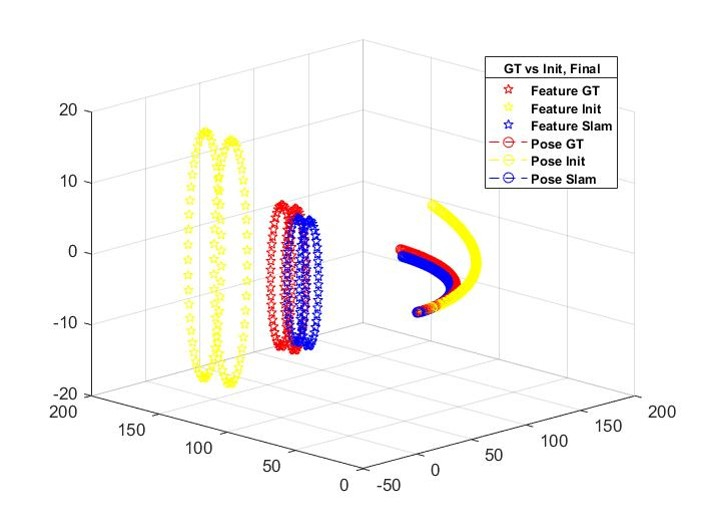
\includegraphics[height=10.3cm]{figures/SimuNpose_simData.jpg}
	\caption{SimuNpose Naive vs Preintegration VIN}
	\label{fig:simuNpose}
\end{figure}

A matlab routine $Main\_simuNpose.m$ was prepared to simulate VIN system and evaluate the performance of VIN with and without Pre-Integration.
Table \ref{tab:table1} shows performance results of Naive VIN vs Pre-integration. The later is much more efficient.
\begin{table}[h!]
	\centering
	\caption{Caption for the table.}
	\begin{tabular}{cc|c|c}
		Num image frames &  & Naive VIN & Pre-Integration\\
		\hline
		10 & Total time & 39.1 [sec] & 4.4 [sec]\\
		{} & $\delta X$ & 4.2 & 15.7\\
		\hline
		20 & Total time & 145.1 [sec] & 9.1 [sec]\\
		{} & $\delta X$ & 7.69 & 3.87\\
		\hline
		100 & Total time & NIL & 44.5 [sec]\\
		{} & $\delta X$ & NIL & 12\\		
	\end{tabular}
	\label{tab:table1}
\end{table}


A simulation run of Pre-integration is shown in Figure \ref{fig:simuNpose}. 


\subsection{Incremental initialization of states}
Direct initialization may lead to errors for long tests. This is probably due to non-linearity in transforming from pre-integrated inertial back to global frame, see equation (\ref{eq:Idt2X_orig_1} - \ref{eq:Idt2X_orig_3}). The problem is solved by incremental introduction of new camera poses. Starting with limited number of frames, obtain optimized robot poses and features. Now introduce new observation, using previously obtained values as initial guess in new optimization, expand state vectors if necessary. Repeat process until all observations are covered. A matlab routine $Main\_inc.m$ was developed to simulate the process, see Fig \ref{fig:preint_init}.\emph{b} for illustration. Note: this is in effect similar to iSam2.

	\begin{figure}[h!]
		\begin{center}\begin{tabular}{cc}
				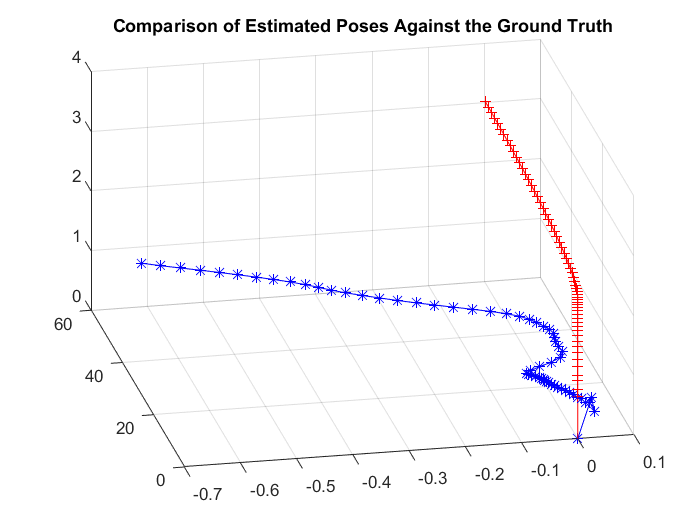
\includegraphics[height=5cm]{figures/simuNpose_error.png} &
				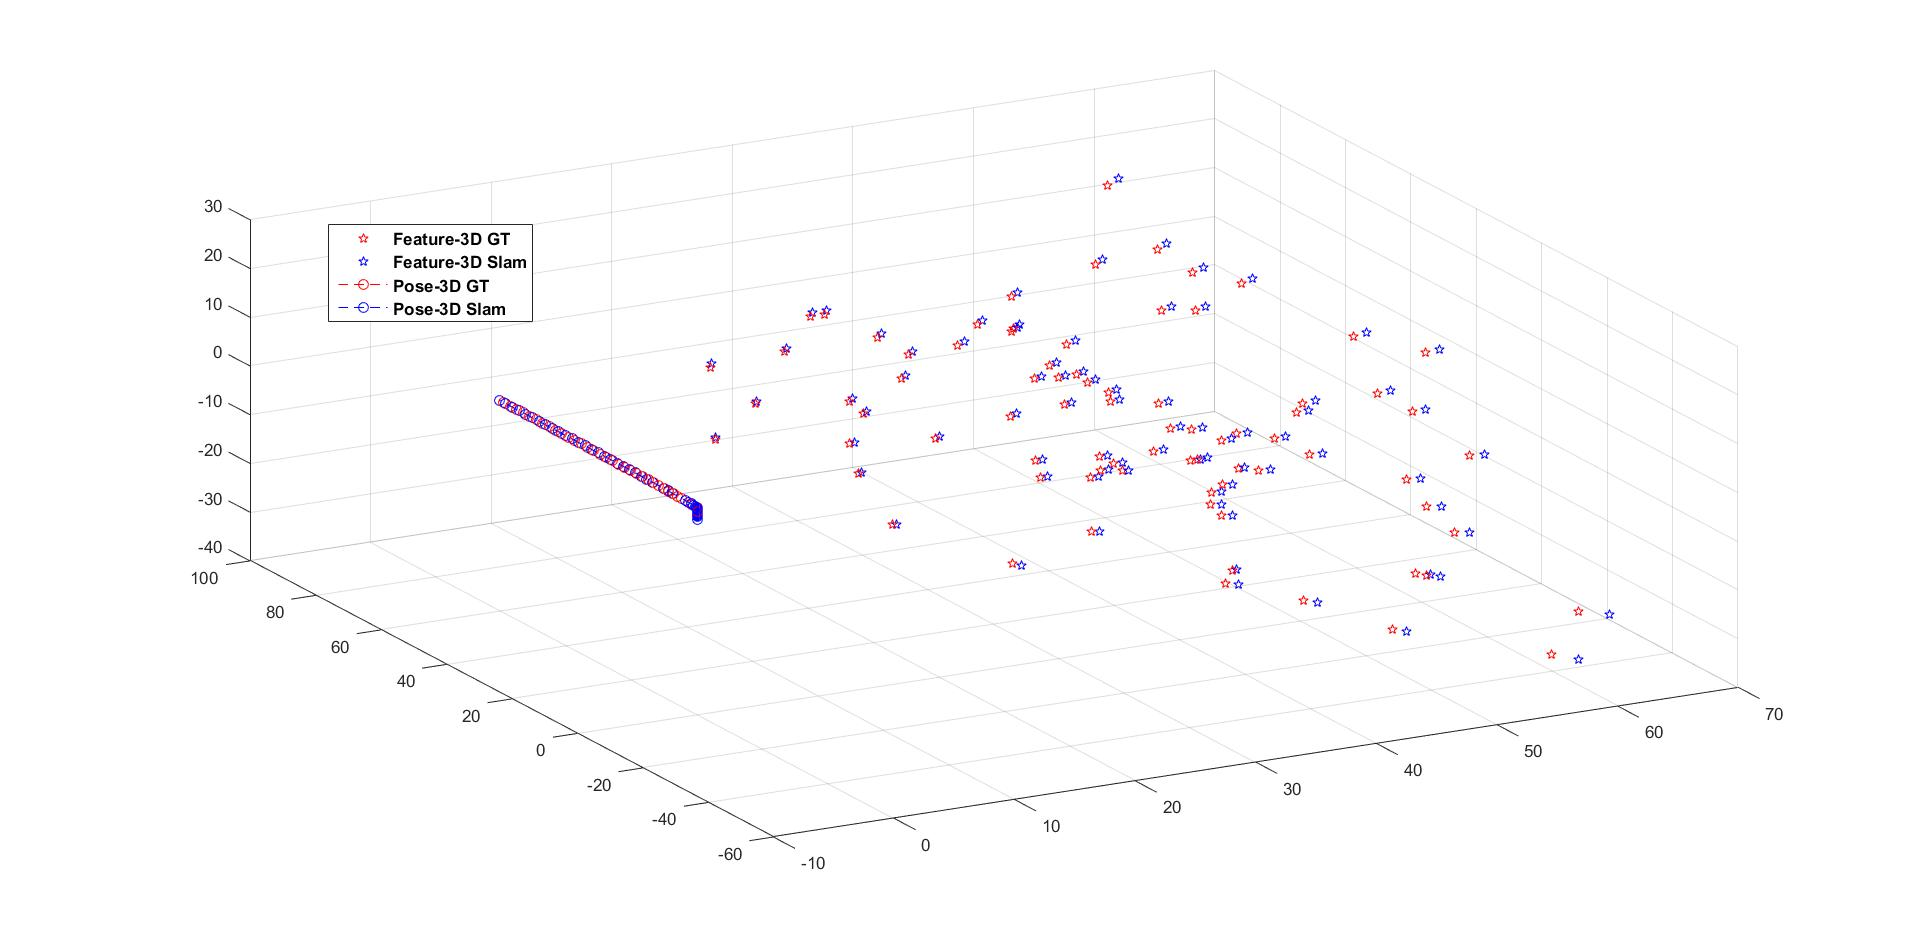
\includegraphics[height=5cm]{Figures/Final_pose-feature_3D_GT-vs-SLAM.jpg}\\				
			\end{tabular}\end{center}
			\caption{\emph{a}) One off initialization , \emph{b}) Incremental initialization } 
			\label{fig:preint_init}
	\end{figure} 

\subsection{Future improvements}
\begin{itemize}
	\item Change parameterization with Manifold \cite{Manifold2015}
	\item Merge Parallax angles into feature representation \cite{ParallaxBA2015}
\end{itemize}
\newpage 
%-----------------------------------------------------------------------------------------
\begin{appendices}
	\lhead{\emph{Appendices}} % 
	\section{Rotation representation -- Euler angles}
	
	\subsection{Rotation matrix}
	\begin{align*}
		R &=R_{x}(\alpha) R_{y}(\beta) R_{z}(\gamma) \nonumber \\
		  &= \begin{pmatrix} 
				1 & 0 & 0 
				\\ 0 & \cos(\alpha) & \sin(\alpha) 
				\\ 0 & -\sin(\alpha) & \cos(\alpha) 
			\end{pmatrix} 
			\begin{pmatrix} 
				\cos(\beta) & 0 & -\sin(\beta) \\ 
				0 & 1 & 0 \\ 
				\sin(\beta) &  0 & \cos(\beta) 
			\end{pmatrix} 
			\begin{pmatrix} 
				\cos(\gamma) & \sin(\gamma) & 0 
				\\ -\sin(\gamma) & \cos(\gamma) &  0 
				\\ 0 & 0 & 1 
			\end{pmatrix} \\	
		\end{align*}
		
	\subsection{Rotation Rate Matrix}
	\begin{align*}
	E &= \begin{pmatrix} 
			1 & 0 & -sin(\beta) \\ 
			0 & cos(\alpha) & cos(\beta)sin(\alpha) \\ 
			0 & -sin(\alpha) & cos(\beta)cos(\alpha) 
		 \end{pmatrix} \\
	\end{align*}
	
	\subsection{Camera frame to Global transform}	
Using the IMU's coordinates at the 1st pose as the global reference frame, the relative position of these two sensors at that time can be related by $\textbf{A}_{u2c}$ and $\textbf{T}_{u2c}$, : 
\begin{eqnarray*}   % do not need dollar signs because eqnarray puts you in math mode
	\textbf{A}_{u2c} & = & (\alpha_{u2c}, \beta_{u2c}, \gamma_{u2c}), \\
	\textbf{T}_{u2c} & = & (x_{u2c}, y_{u2c}, z_{u2c})
\end{eqnarray*}

And at the following poses, given IMU's states ($\textbf{R}^u_i$ and $\textbf{T}^u_i$), the camera's states ($\textbf{R}^c_i$ and $\textbf{T}^c_i$) can be obtained according to this formula:

\begin{align*}
\textbf{R}^c_i &= \textbf{R}_{u2c} \textbf{R}^u_i \\
\textbf{p}^c_i &= \textbf{p}^u_i + {\textbf{R}^u_i}'  \textbf{T}_{u2c}  
\end{align*} 
	
\section{Preintegration VIN Jacobian}
\label{apn:preintVin}
\subsection{Jacobian of Inertial Delta to X}
Based on the composition of $H(\textbf{x})$, the corresponding Jacobian matrix can be calculated. 

For camera observations of $(u_{ij}, v_{ij}, d_{ij})$ which represent the observation of the $i$th feature at the $j$th camera pose, 
\begin{align}
\frac{\partial u_{ij}}{\partial \textbf{F}_{ij}} &= [f/z_{ij}, 0, -fx_{ij}/z^2_{ij}] \\
\frac{\partial v_{ij}}{\partial \textbf{F}_{ij}} &= [0, f/z_{ij}, -fy_{ij}/z^2_{ij}] \\
\frac{\partial d_{ij}}{\partial \textbf{F}_{ij}} &= [0, 0, 1] \\
\frac{\partial \textbf{F}_{ij}}{\partial \textbf{A}_{j}} &= R_{u2c} \frac{\partial R_{j}}{\partial \textbf{A}_{j}} (\textbf{F}_{i1} - \textbf{p}_{j}) \\
\frac{\partial \textbf{F}_{ij}}{\partial \textbf{T}_{j}} &= -R_{u2c} R_{j} \\
\frac{\partial \textbf{F}_{ij}}{\partial \textbf{A}_{u2c}} &= \frac{\partial R_{u2c}}{\partial \textbf{A}_{u2c}} R_{j}(\textbf{F}_{i1} - R'_{j} \textbf{T}_{u2c} - \textbf{p}_{j}) \\
\frac{\partial \textbf{F}_{ij}}{\partial \textbf{T}_{u2c}} &= -R_{u2c}\\
\frac{\partial \textbf{F}_{ij}}{\partial \textbf{F}_{i1}} &= R_{u2c} R_{j} 
\end{align}

For $d\text{p}^+_{i}$,

\begin{align}
%%%%%%%
% dp = R1 * (T2-T1-v1*dt-0.5*g*dt*dt) - ddpdbf*dbf - ddpdbw*dbw;
\frac{\partial d\textbf{p}^+_{i}}{\partial \textbf{A}_{i}} &= \frac{\partial R_i}{\partial \textbf{A}_i} ( \textbf{p}_{i+1} - \textbf{p}_i - \textbf{v}_i \triangle t - \frac{1}{2} \textbf{g}^{\mathrm{n}} {(\triangle t)}^2 ) \\
\frac{\partial d\textbf{p}^+_{i}}{\partial \textbf{p}_{i}} &= -R_i \\
\frac{\partial d\textbf{p}^+_{i}}{\partial \textbf{p}_{i+1}} &= R_i \\
\frac{\partial d\textbf{p}^+_{i}}{\partial \textbf{v}_{i}} &= -R_i \triangle t \\
\frac{\partial d\textbf{p}^+_{i}}{\partial \textbf{g}} &= -\frac{1}{2} R_i {\triangle t}^2 \\
\frac{\partial d\textbf{p}^+_{i}}{\partial \textbf{b}_f} &= - \frac{\partial \triangle \textbf{p}^+_t}{\partial \textbf{b}_f}\\
\frac{\partial d\textbf{p}^+_{i}}{\partial \textbf{b}_\omega} &= - \frac{\partial \triangle \textbf{p}^+_t}{\partial \textbf{b}_\omega}
\end{align}
%%%%%

For $d\text{v}_{i}$,

\begin{align}
% dv = R1 * (v2-v1-g*dt) - jddvdbf*(bf-bf0) - jddvdbw*(bw-bw0)
\frac{\partial d\textbf{v}_{i}}{\partial R_{i}} &= \frac{\partial R_i}{\partial \textbf{A}_i} (\textbf{v}_{i+1} - \textbf{v}_i - \textbf{g}^{\mathrm{n}} \triangle t) \\
\frac{\partial d\textbf{v}_{i}}{\partial \textbf{v}_{i}} &= -R_i \\
\frac{\partial d\textbf{v}_{i}}{\partial \textbf{v}_{i+1}} &= R_i \\
\frac{\partial d\textbf{v}_{i}}{\partial \textbf{g}} &= -R_i \triangle t \\
\frac{\partial d\textbf{v}_{i}}{\partial \textbf{b}_f} &= - \frac{\partial \triangle \textbf{v}_t}{\partial \textbf{b}_f}\\
\frac{\partial d\textbf{v}_{i}}{\partial \textbf{b}_\omega} &= - \frac{\partial \triangle \textbf{v}_t}{\partial \textbf{b}_\omega}
\end{align}

For $d\textbf{A}_{i}$,
\begin{align}
% [a,b,g] = fnABG5R(Ru2*(Ru1)'); dphi = [a;b;g] - ddphidbw*dbw 
\frac{\partial \triangle \textbf{A}_{i}}{\partial \textbf{A}_{i}} &= \frac{\partial fn}{\partial R} R_{i+1} \frac{\partial R_i}{\partial \textbf{A}_{i}}\\
\frac{\partial \triangle \textbf{A}_{i}}{\partial \textbf{A}_{i+1}} &= \frac{\partial fn}{\partial R} \frac{\partial R_{i+1}}{\partial \textbf{A}_{i+1}} R_{1} \\
\frac{\partial \triangle \textbf{A}_{i}}{\partial \textbf{b}_\omega} &= - \frac{\partial \triangle \textbf{A}_t}{\partial \textbf{b}_\omega}
\end{align}

where $d\textbf{P}_{i} = (dx_{i}, dy_{i}, dz_{i}) $,
$d\textbf{v}_{i} = (dvx_{i}, dvy_{i}, dvz_{i}) $, and
$d\textbf{A}_{i} = (d\alpha_{i}, d\beta_{i}, d\gamma_{i}) $.

\section{Naive VIN}
\label{apn:naiveVin}
The measurements model $H(\textbf{x})$ in Naive VIN can be broken into the following three parts:

\begin{align}
%E_{ij} &= \begin{pmatrix} 1 & 0 & -sin(\beta) \\ 0 & cos(\alpha) & cos(\beta)sin(\alpha) \\ 0 & -sin(\alpha) & cos(\beta)cos(\alpha) \end{pmatrix} \\
\omega_{ij} &= E_{ij} (\textbf{A}_{(i+1)j} - \textbf{A}_{ij})/\triangle t + \textbf{b}_w \\
\textbf{f}_{ij} &= R_{ij} ((\textbf{v}_{(i+1)j} - \textbf{v}_{ij}) / \triangle t - \textbf{g}^{\mathrm{n}}) + \textbf{b}_f \\
\textbf{bZeros} &= \textbf{p}_{(i+1)j} - \textbf{p}_{ij} - \textbf{v}_{ij} \triangle t
\end{align}

where $i = 0,..., K-1$, and $R_{ij}, E_{ij} ( = \begin{pmatrix} 1 & 0 & -\sin(\beta_{ij}) \\ 0 & \cos(\alpha_{ij}) & \cos(\beta_{ij})\sin(\alpha_{ij}) \\ 0 & -\sin(\alpha_{ij}) & \cos(\beta_{ij})\cos(\alpha_{ij}) \end{pmatrix}) $ correspond to the rotation matrix and rotation rate matrix for the IMU at the time step $i$ since the $j$th key camera frame respectively.

Putting all items together, $H(\textbf{x})$ can be written as:

\begin{align} % R_{01} * ((\textbf{v}_{11} - \textbf{v}_{01}) / \triangle t - \textbf{g}) + \textbf{b}_f, E_i*(	extbf{A}_{0N} - \textbf{A}_{(K-1)(N-1)})/\triangle t + \textbf{b}_w, 
H(\textbf{x}) &= (H_{camera}(\textbf{x}), H_{IMUraw}(\textbf{x}), H_{Tv}(\textbf{x})) \nonumber \\
=& (\overbrace{{u}_{11}, {v}_{11}, ... , {u}_{M1}, {v}_{M1}, ..., {u}_{1N}, {v}_{1N}, ... , {u}_{MN}, {v}_{MN}}^{M \times N \times 2}, \nonumber \\ 
& \overbrace{\omega\textbf{f}_{01}, \omega\textbf{f}_{11}, ... , \omega\textbf{f}_{(K-1)1}, ..., \omega\textbf{f}_{0(N-1)}, \omega\textbf{f}_{1(N-1)}, ... , \omega\textbf{f}_{(K-1)(N-1)}}^{K \times (N-1) \times 6}, \nonumber \\
& \overbrace{\textbf{p}_2 - \textbf{p}_{1} - \textbf{v}_{1} \triangle t, \textbf{p}_{3} - \textbf{p}_{2} - \textbf{v}_{2} \triangle t, ... , \textbf{p}_{(N-1)K+1} - \textbf{p}_{(N-1)K} - \textbf{v}_{(N-1)K} \triangle t}^{K \times (N-1) \times 3}) \nonumber \\
=& (\overbrace{f * x_{11} / z_{11} + cx_0, f * y_{11} / z_{11} + cy_0, ... , f * x_{MN} / z_{MN} + cx_0, f * y_{MN} / z_{MN} + cy_0, }^{M \times N \times 2}, \nonumber \\ 
& \overbrace{E_i*(\textbf{A}_{11} - \textbf{A}_{01})/\triangle t + \textbf{b}_w, ..., R_{(K-1)(N-1)} * ((\textbf{v}_{0N} - \textbf{v}_{(K-1)(N-1)}) / \triangle t - \textbf{g}^{\mathrm{n}}) + \textbf{b}_f}^{K \times (N-1) \times 6}, \nonumber \\
& \overbrace{\textbf{p}_2 - \textbf{p}_{1} - \textbf{v}_{1} \triangle t, \textbf{p}_{3} - \textbf{p}_{2} - \textbf{v}_{2} \triangle t, ... , \textbf{p}_{(N-1)K+1} - \textbf{p}_{(N-1)K} - \textbf{v}_{(N-1)K} \triangle t}^{K \times (N-1) \times 3}) 
\end{align}

\subsection{Jacobian Matrix}

Based on the composition of $H(\textbf{x})$, the corresponding Jacobian matrix can be calculated. 

For camera observations of $(u_{ij}, v_{ij}, d_{ij})$ which represent the observation of the $i$th feature at the $j$th camera pose, 
\begin{align}
% bZeros: \textbf{bZeros} &= \textbf{T}_{i+1} - \textbf{T}_{i} - \textbf{v}_{i} \triangle t 
\frac{\partial u_{ij}}{\partial \textbf{F}_{ij}} &= [f/z_{ij}, 0, -fx_{ij}/z^2_{ij}] \\
\frac{\partial v_{ij}}{\partial \textbf{F}_{ij}} &= [0, f/z_{ij}, -fy_{ij}/z^2_{ij}] \\
\frac{\partial d_{ij}}{\partial \textbf{F}_{ij}} &= [0, 0, 1] \\
%% X = Ru2c * Ru * (X0 - Ru'* Tu2c - Tu)
%%   = Ru2c * Ru * (X0 - Tu)- Ru2c * Tu2c
\frac{\partial \textbf{F}_{ij}}{\partial \textbf{A}_{0j}} &= R_{u2c} \frac{\partial R_{0j}}{\partial \textbf{A}_{0j}} (\textbf{F}_{i1} - \textbf{p}_{0j}) \\
\frac{\partial \textbf{F}_{ij}}{\partial \textbf{p}_{0j}} &= -R_{u2c} R_{0j} \\
\frac{\partial \textbf{F}_{ij}}{\partial \textbf{A}_{u2c}} &= \frac{\partial R_{u2c}}{\partial \textbf{A}_{u2c}} R_{0j}(\textbf{F}_{i1} - R'_{0j} \textbf{T}_{u2c} - \textbf{p}_{0j}) \\
\frac{\partial \textbf{F}_{ij}}{\partial \textbf{T}_{u2c}} &= -R_{u2c}\\
\frac{\partial \textbf{F}_{ij}}{\partial \textbf{F}_{fi}} &= R_{u2c} R_{0j} 
\end{align}

For $\omega_{ij}$,

\begin{align}
%%%%%%%
% \omega_i &= E_i (\textbf{A}_{i+1} - \textbf{A}_i)/\triangle t + \textbf{b}_w
%\left \{
%\begin{align*}
\frac{\partial \omega_{ij}}{\partial \textbf{A}_{ij}} &= \frac{\partial E_{ij}}{\partial \textbf{A}_{ij}} (\textbf{A}_{(i+1)j} - \textbf{A}_{ij})/\triangle t + E_{ij} (- \frac{\partial \textbf{A}_{ij}}{\partial \textbf{A}_{ij}})/\triangle t \nonumber \\
&= (\frac{\partial E_{ij}}{\partial \textbf{A}_{ij}} (\textbf{A}_{(i+1)j} - \textbf{A}_{ij}) - E_{ij})/\triangle t \\
\frac{\partial E_{ij}}{\partial \textbf{A}_{ij}} &= [\frac{\partial E_{ij}}{\partial \alpha_{ij}}, \frac{\partial E_{ij}}{\partial \beta_{ij}}, \frac{\partial E_{ij}}{\partial \gamma_{ij}}] \\
%\frac{\partial \omega_{ij}}{\partial \alpha_{ij}} &= \frac{\partial E_{ij}}{\partial \alpha_{ij}}*(\textbf{A}_{(i+1)j} - \textbf{A}_{ij})/\triangle t + E_{ij}*(- \frac{\partial \textbf{A}_{ij}}{\partial \alpha_{ij}})/\triangle t \\
%\frac{\partial \omega_{ij}}{\partial \beta_{ij}} &= \frac{\partial E_{ij}}{\partial \beta_{ij}}*(\textbf{A}_{(i+1)j} - \textbf{A}_{ij})/\triangle t + E_{ij}*(- \frac{\partial \textbf{A}_{ij}}{\partial \beta_{ij}})/\triangle t \\
%\frac{\partial \omega_{ij}}{\partial \gamma_{ij}} &= \frac{\partial E_{ij}}{\partial \gamma_{ij}}*(\textbf{A}_{(i+1)j} - \textbf{A}_{ij})/\triangle t + E_{ij}*(- \frac{\partial \textbf{A}_{ij}}{\partial \gamma_{ij}})/\triangle t \\
\frac{\partial \omega_{ij}}{\partial \textbf{A}_{(i+1)j}} &= E_{ij} \frac{\partial \textbf{A}_{(i+1)j}}{\partial \textbf{A}_{(i+1)j}}/\triangle t \\
&= E_{ij}/\triangle t \\
\frac{\partial \omega_{ij}}{\partial b_{\omega}} &= I_{3\times 3} 
%\right.
\end{align}
%%%%%

For $\textbf{f}_{ij}$,

\begin{align}
% a_i \textbf{a}_i &= R_i ((\textbf{v}_{i+1} - \textbf{v}_i) / \triangle t - \textbf{g}) + \textbf{b}_f 
\frac{\partial \textbf{f}_{ij}}{\partial \textbf{A}_{ij}} &= \frac{\partial R_{ij}} {\textbf{A}_{ij}} ((\textbf{v}_{i+1} - \textbf{v}_i) / \triangle t - \textbf{g}) \\
\frac{\partial R_{ij}}{\partial \textbf{A}_{ij}} &= [\frac{\partial R_{ij}}{\partial \alpha_{ij}}, \frac{\partial R_{ij}}{\partial \beta_{ij}}, \frac{\partial R_{ij}}{\partial \gamma_{ij}}] \\
\frac{\partial \textbf{f}_{ij}}{\partial \textbf{v}_{(i+1)j}} &= R_{ij} / \triangle t \\
\frac{\partial \textbf{f}_{ij}}{\partial \textbf{v}_{ij}} &= - R_{ij} / \triangle t \\
\frac{\partial \textbf{f}_{ij}}{\partial \textbf{g}} &= - R_{ij}\\
\frac{\partial \textbf{f}_{ij}}{\partial b_{f}} &= I_{3\times 3} 
\end{align}

For $\textbf{bZeros}_{ij}$,
\begin{align}
% bZeros: \textbf{bZeros} &= \textbf{T}_{i+1} - \textbf{T}_{i} - \textbf{v}_{i} \triangle t 
\frac{\partial \textbf{bZeros}_{ij}}{\partial \textbf{p}_{(i+1)j}} &= I_{3\times 3} \\
\frac{\partial \textbf{bZeros}_{ij}}{\partial \textbf{p}_{ij}} &= - I_{3\times 3} \\
\frac{\partial \textbf{bZeros}_{ij}}{\partial \textbf{v}_{ij}} &= - I_{3\times 3} \triangle t  
\end{align}


	
\end{appendices}

\newpage 
%-----------------------------------------------------------------------------------------
%----------------------------------------------------------------------------------------
%	BIBLIOGRAPHY
%----------------------------------------------------------------------------------------
\section{Bibliography}
\label{Bibliography}

\lhead{\emph{PreIntegration}} % Change the page header to say "Bibliography"

\bibliographystyle{unsrtnat} % Use the "unsrtnat" BibTeX style for formatting the Bibliography

\bibliography{vins} % The references (bibliography) information are stored in the file named "Bibliography.bib" Bibliography

\end{document}

